\chapter{Identifying impactful fusion genes: fusion expression
  analysis}


\section{Motivation}
Acquisition of increasing numbers of somatic mutations on a rapid
timescale and in a heterogeneous fashion across different cells within
a tumor or pre-tumor tissue, is widespread and occurs in most cancer
types. Resulting mutations are sufficient to induce tumorigenesis and
also to drive tumor progression and metastasis. This is done
classically through the activation of proto-oncogenes and through the
deactivation of tumor suppressor genes.


There are several specific pathways by which mutations can be induced
and several corresponding classes of mutations\cite{stratton_cancer_2009}. One class is
large-scale genomic rearrangement, which involves the breaking and
possible rejoining of multiple-megabase sections of DNA.


When large genomic regions dislocate, they may often rejoin in a
predictable fashion to regions either on other chromosomes or within
the same chromosome (translocations).  If there are genic regions
spanning the genomic breakpoints, RNA messages may be transcribed that
contain two genes from two constituent chromosomes. Such messages, if
translated, become fusion genes (FGs).


Due to fragile regions in DNA, specific FGs may be formed to a
significant extent in certain tissues during
tumorigenesis\cite{yunis_constitutive_1984}. In chronic myeloid
leukemia (CML), a fusion between breakpoint cluster region (BCR) and
Abelson murine leukemia (ABL) virus genes leads to the recurrent
BCR-ABL fusion which is present in a large percentage of CML
patients. This fusion is known to have potential to transform normal
cells into cells with tumor characteristics, and has been successfully
targeted by Imatinib, one of the world’s first successful targeted
therapies in terms of extending patient overall survival time. Several
similar examples have been discovered; identifying FGs is thus of
primary interest \cite{chin_cancer_2011}. 

One goal of major consortium efforts such as The Cancer Genome Atlas
(TCGA)\cite{weinstein_cancer_2013} and The Cancer Cell Line
Encyclopedia (CCLE)\cite{barretina_cancer_2012} is detecting recurrent
fusion genes from different caner types based on sequencing
information. Recently, for example, recurrent receptor tyrosine kinase
fusions were detected in gliomas\cite{_comprehensive_2015}.

One mechanism whereby fusion genes may have impact on tumor tissue is
via the induced expressional deregulation (ED) of the constituents. In particular, a sequence may be placed under the control of regulatory regions that were not originally meant for a sequence, resulting in, for example, the constitutive expression of a growth-factor related protein domain \todo{citation for deregulation}, leading to oncogenesis or tumor progression. 


\section{Existing Impact-Assessment Strategies}
\subsection{Detection}
Typically, fusions are detected from RNA-sequencing (RNA-seq) reads,
which are produced due to its relatively low cost compared to whole
genome sequencing and high interpretability. Several computational
tools to detect fusions from RNA-seq reads exist. Most identify fusion
junctions (FJs), which are the breakpoints of the associated
genomic translocations.


Tools identify FJs in three steps: (1) finding chimeric reads (CRs), which is a single read with two portions aligning to two separate genomic locations, (2) aggregating chimeric reads into candidate fusion junctions through realignment-based grouping, and (3) filtering candidate FJs based on heuristic filters. 

While simple in concept, identifying FJs is a problematically error-prone process. Firstly, incorrect read mapping leads to spurious CRs. Incorrect mapping is often a result of repetitive regions in the genome such as germline segmental duplications. Secondly, even if reads are correctly aligned, false positives may be generated by read-through events, where genomically adjacent genes are erroneously transcribed into one RNA message or reverse transcriptase template-switching events/ trans-splicing. These produce low but detectable baseline levels of fusion genes in wild-type cells, but are usually not of interest in cancer sequencing efforts as they are not causally involved in tumorigenesis, cancer progression, or metastasis\cite{gingeras_implications_2009}. 

Thus, candidate FJs must be filtered aggressively by heuristics based on knowledge of the above. One problem is that it’s not clear exactly which heuristics to use; many heuristics based on ignoring FGs in repetitive regions, for example, may filter real fusions\cite{kumar_identifying_2016}. Another is that given a set of heuristic filters, it’s not clear how to best combine the heuristics in a way that’s generalizable to most FG discovery use cases. This is due in part to the wide range of genomic instability that tumors from different tissues have exhibited. A symptom of this is that Machine learning-based classifiers tuned on representative datasets have issues generalizations to new tumor types. The high false-positive rate stymies further discovery and assessment of FGs. 

FJ identification is also a very computationally-intensive process, as every read must be split in a number of ways and positions and matched against all possible regions of the genome through alignment during CR-finding steps. One of the reasons for this is that existing fusion discovery methods use computationally intensive first-generation alignment algorithms. 

\subsection{Expression Quantification}

As ED is a major mechanism by which fusion genes impact tumors and patients, assessing whether an individual fusion detected has also led to ED is a goal for prioritizing fusions for per-patient impact and for further mechanistic study.

Unfortunately, there is no currently established method of doing so in a high-throughput, unbiased fashion. Three methods currently exist:

\subsubsection{Constituent Gene Summing}

One approach to assessing whether a fusion gene or transcript is expressionally deregulated is by summing the expression estimates of its constituent transcripts. If the sum of these expression estimates substantially deviates from the same quantity in sample(s) without the fusion, it is concluded that the fusion has led to ED.

However, this is inaccurate due to details involving how much of each constituent transcript makes up the fusion. In particular, a fusion gene can consist of the entire transcripts of the constituents bound, or it can consist of as little as a few bases of each gene. This wide discrepancy leads to the lack of robustness of this method without substantial additional human assessment, which is undesirable as the purpose of high-throughput and automated assessment methods is to minimize human input. The presence of large numbers of false-positive fusions exacerbates this necessity of visual inspection as well.

\begin{center}
\begin{figure}\centering
  \parbox{.9\textwidth}{\centering
\noindent 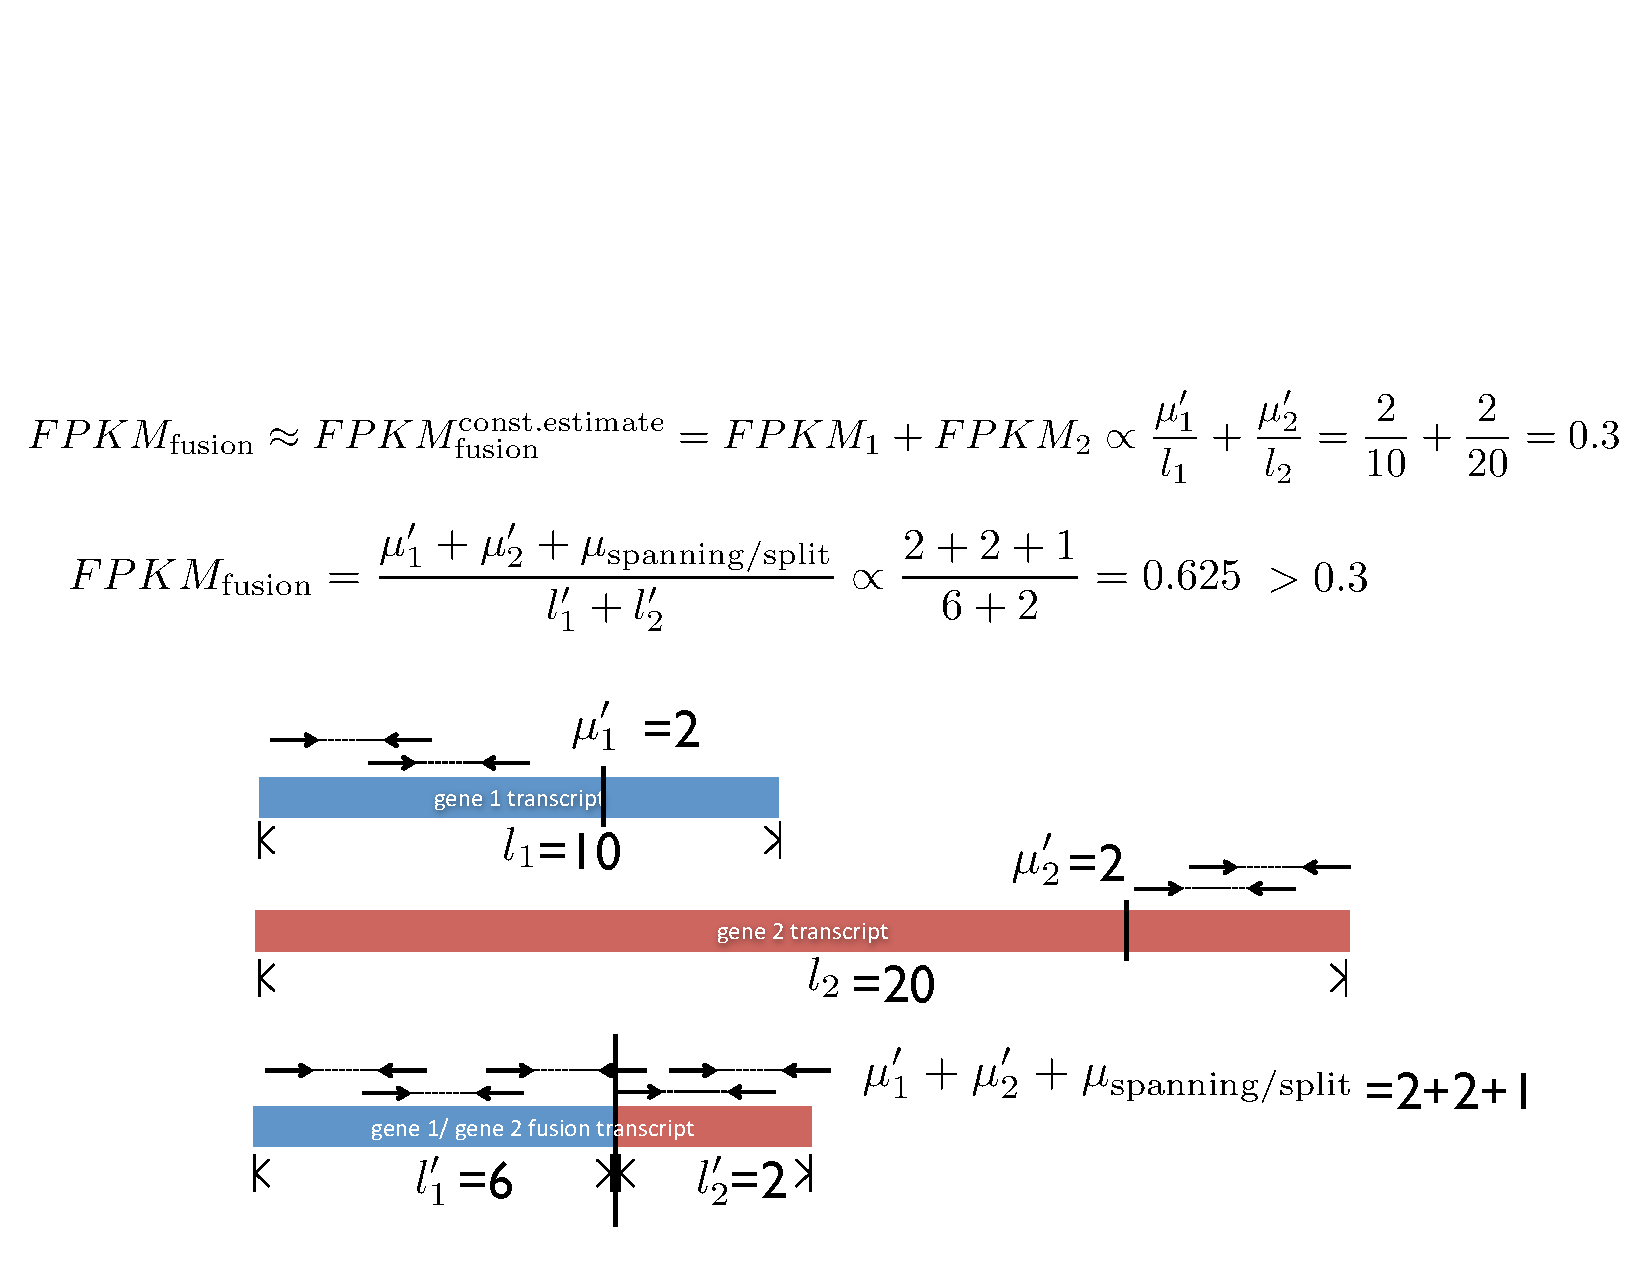
\includegraphics[width=.9\textwidth]{/Users/ijoseph/Documents/Work/Graduate-Thesis/TeX/figures/ch3_1.pdf}
    \caption{Illustration of inaccuracy of constituent summing method ($\mathrm{FPKM}_{\mathrm{fusion}}^{\mathrm{const.estimate}}$) for estimating expression of fusion transcript ($\mathrm{FPKM}_\mathrm{fusion}$), resulting in underestimation by a factor of $2$ }}.
\end{figure}
\end{center}


\subsubsection{Per-Exon Inspection}

A related but distinct method of assessing fusion genes is comparison between fusion-present and fusion-absent samples by visually inspecting the per-exon expression of the constituent transcripts. While not susceptible to the problems of the summing method in terms of misestimation, this is even more labor-intensive as it is completely not automated.

\subsubsection{Counting Junction-Spanning Reads}

One automated approach to assessing fusion expression estimation is by counting the number of reads supporting the fusion junction. In particular, a read can \textit{support} a fusion junction by being a \textit{spanning read} (PR) or \textit{split read} (LR). A PR is a paired-end read wherein one end maps to one transcript and another maps to a genomically distal genomic region, whereas an LR is a read wherein a portions of one read (if applicable) map to at least two distinct genomic regions.

Some method of counting these reads is a common method of prioritizing fusions; however, this is very susceptible to multi-mapping reads. In particular, if a junction region is repeated in another section of the genome, reads could spuriously seem to strongly support a fusion, whereas in reality the reads were produced by different regions altogether. Thus, this method can be inaccurate. 





% We propose an improved method for FG discovery based on pseudoalignment\cite{bray_near-optimal_2016}. This method achieves high specificity based on ?, and is vastly more computationally efficient than previous methods via the use of pseudoalignment, which uses exact-hashing of k-mers. 







